\documentclass[supercite]{HustGraduPaper}

% ── 个人信息 ──────────────────────────────────────────────
\title{MoS$_2$ 转角同质结的制备与表征}
\author{程远耀}
\date{\today}
\school{物理学院}
\classnum{物理强基2201班}          % 填写专业班级
\stunum{U202210214}          % 填写学号
\instructor{张卜天}

% ── 额外宏包 ──────────────────────────────────────────────
\usepackage{xltxtra}
\usepackage{bm}
\usepackage{siunitx}         % 单位排版，如 \SI{0.316}{nm}
\usepackage{subcaption}      % 子图
\usepackage{multirow}        % 表格跨行
\usepackage{booktabs}        % 三线表

% 图片搜索路径（绝对路径，支持从任意目录编译）
\graphicspath{
  {../../angle_cnn/outputs/}
  {../../data/}
  {../../angle_cnn/docs/figures/literature/pmc10603799/}
  {../../angle_cnn/docs/figures/literature/pmc7195481/}
  {Figures/}
  {/home/cyy2837192872/tmdc-project/angle_cnn/outputs/}
  {/home/cyy2837192872/tmdc-project/data/}
  {/home/cyy2837192872/tmdc-project/angle_cnn/docs/figures/literature/pmc10603799/}
  {/home/cyy2837192872/tmdc-project/angle_cnn/docs/figures/literature/pmc7195481/}
  {/home/cyy2837192872/tmdc-project/thesis/hust_bachelor_cse/Figures/}
}

\begin{document}

% ══════════════════════════════════════════════════════════
% 封面与声明页
% ══════════════════════════════════════════════════════════
\maketitle
\statement

\clearpage
\pagenumbering{Roman}

% ══════════════════════════════════════════════════════════
% 中文摘要
% ══════════════════════════════════════════════════════════
\begin{cnabstract}{MoS$_2$；转角同质结；moiré 超晶格；卷积神经网络；AFM 表征}

转角二维材料通过层间旋转形成 moiré 超晶格，其物理性质对转角精度极为敏感。本文建立了从物理仿真到深度学习的 MoS$_2$ 转角自动提取 pipeline。

仿真方面，基于 moiré 倒格矢差模型直接生成 moiré 包络，并引入连续晶格重构模型（strength 线性插值）消除传统分段函数在 $\theta = 2^{\circ}$ 处的不连续性，使小角度三角畴结构与大角度正弦调制之间的过渡与实验观测一致。在此基础上构建了 $5\times10^4$ 样本的仿真数据集，模拟轻敲模式 AFM 三通道（height / phase / amplitude），退化链包含 TITAN~70 探针卷积、仿射畸变、$1/f$ 噪声等 8 种物理退化。

深度学习方面，采用改造 ResNet 骨干（$3{\times}3$ 首层卷积、Huber Loss、Mixup 数据增强）训练 CNN 回归模型，推理阶段通过 MC Dropout 提供不确定性估计。在公平对比评测中（CNN 用 $128{\times}128$ 训练裁剪，FFT 用 $512{\times}512$ 重算高度图），FFT 平均误差更低（MAE $\approx 0.049^{\circ}$ vs.\ CNN $\approx 0.094^{\circ}$），但 CNN 在低分辨率端到端推理、畸变鲁棒性及不确定性量化方面具有不可替代的优势，二者形成互补。

实验方面已完成 MoS$_2$ 机械剥离与 SiO$_2$/Si 衬底转移。

\end{cnabstract}

% ══════════════════════════════════════════════════════════
% 英文摘要
% ══════════════════════════════════════════════════════════
\begin{enabstract}{MoS$_2$; twisted homojunction; moiré superlattice; convolutional neural network; AFM characterization}

Twisted two-dimensional materials form moiré superlattices whose physical properties depend critically on twist-angle accuracy. This work builds a simulation-to-learning pipeline for automated twist-angle extraction from MoS$_2$ moiré patterns.

On the simulation side, moiré envelopes are generated via a reciprocal-space difference construction. A continuous lattice reconstruction model with linear \textit{strength} interpolation is introduced to eliminate the artificial discontinuity at $\theta = 2^{\circ}$ in conventional piecewise models, yielding a smooth transition between triangular domain structures at small angles and sinusoidal modulation at large angles, consistent with experimental observations. A synthetic dataset of $5\times10^4$ multichannel (height / phase / amplitude) AFM-like images at $128{\times}128$ pixels is produced, with an 8-step degradation chain including TITAN~70 probe convolution, affine drift, $1/f$ noise, and other physically motivated distortions.

On the deep-learning side, a modified ResNet backbone ($3{\times}3$ stem convolution, Huber loss, Mixup augmentation) is trained for regression, with MC Dropout providing uncertainty estimates at inference. Under a fair evaluation protocol (CNN on $128{\times}128$ crops, FFT on re-synthesized $512{\times}512$ height maps), FFT achieves a lower MAE ($\approx 0.049^{\circ}$ vs.\ $\approx 0.094^{\circ}$). Nevertheless, CNN offers irreplaceable advantages in end-to-end inference on low-resolution input, robustness to distortions, and built-in uncertainty quantification, making the two methods complementary.

Experimentally, MoS$_2$ exfoliation and transfer to SiO$_2$/Si substrates have been completed.

\end{enabstract}

% ══════════════════════════════════════════════════════════
% 目录
% ══════════════════════════════════════════════════════════
\tableofcontents[pagenum=true]

\clearpage
\pagenumbering{arabic}

% ══════════════════════════════════════════════════════════
% 第1章  绪论
% ══════════════════════════════════════════════════════════
\section[绪论]{绪论\textsuperscript{*}}

\subsection{研究背景与意义}

自 2018 年 Cao 等人在魔角扭转双层石墨烯中发现莫特绝缘体和非传统超导性以来，转角二维材料体系（"转角电子学"，Twistronics）成为凝聚态物理最活跃的研究前沿之一\cite{cao2018unconventional}。通过在范德华材料双层结构中引入特定的层间转角 $\theta$，两层晶格形成具有纳米尺度超周期的 moiré 超晶格，其周期 $L$ 由转角和晶格常数 $a$ 决定：
\begin{equation}
  L = \frac{a\sqrt{3}}{4\sin(\theta/2)}
  \label{eq:moire_period}
\end{equation}

moiré 超晶格在倒空间产生微型布里渊区，使能带被折叠压缩，在特定"魔角"附近出现极窄的平带，从而极大增强电子关联效应，涌现出超导、莫特绝缘、铁磁等多种强关联量子相。McGilly 等人利用压电力显微镜直接可视化了 moiré 超晶格的畴结构，揭示了晶格重构的空间分布\cite{mcgilly2020visualization}。

过渡金属二硫化物（TMDC）体系，尤其是 MoS$_2$ 转角同质结，因其具有直接带隙（$E_g \approx 1.8\,\mathrm{eV}$）、强自旋-轨道耦合和空间反演对称性破缺等特征，在转角研究中具有独特优势。小角度（$\theta < 2^{\circ}$）MoS$_2$ 转角双层在 moiré 超晶格中形成 AB 和 BA 两类三角形堆叠域，伴随显著的晶格重构和压电极化\cite{weston2020atomic}，为研究激子局域化、层极化和拓扑相变提供了重要平台。Liao 等人实现了大面积 MoS$_2$ 同质结的精确转角控制，为批量制备提供了工艺基础\cite{liao2020precise}。

\subsection{转角精度表征的挑战}

转角精度直接决定 moiré 周期和体系的物理性质。以 MoS$_2$ 为例，转角从 $1.0^{\circ}$ 变化到 $1.1^{\circ}$ 时，moiré 周期从 $15.7\,\mathrm{nm}$ 缩短到 $14.3\,\mathrm{nm}$，对应的能带结构发生定性变化。因此，精确表征转角是制备与研究的核心需求。

目前常用的转角表征手段包括：光学边缘法（精度 $1^{\circ}$--$2^{\circ}$，仅用于初步估计）、Raman 光谱辅助定标（精度 $0.5^{\circ}$--$1^{\circ}$）、AFM moiré 成像结合 FFT 提取（精度 $0.05^{\circ}$--$0.2^{\circ}$）以及 SHG 极化扫描（精度 $< 0.1^{\circ}$）。其中，AFM 图像结合 FFT 分析是目前实验室最常用的方法，但其精度受到 AFM 扫描中热漂移和压电非线性引入的仿射畸变的严重制约。传统 FFT 方法在含畸变条件下误差增大至数度量级，远超实验需求。Engelke 等人发展了扭转力显微镜方法，可在原子尺度直接测量 moiré 畴结构，但对仪器要求极高\cite{engelke2024torsional}。

\subsection{相关工作}

在扫描探针表征方面，Liao 等在大面积 MoS$_2$ 同质结工作中给出了 AFM 形貌图，验证了样品表面与界面质量，说明 MoS$_2$ 扭转体系具备 AFM 形貌表征的实验可行性\cite{liao2020precise}。McGilly 等采用压电响应力显微镜（PFM，AFM 家族模式）直接可视化了 moiré 超晶格的实空间网络\cite{mcgilly2020visualization}。在深度学习应用于材料表征方面，近年来已有将 CNN 用于原子图像自动分析\cite{o2019atomistic}、STM 图谱分类\cite{ziletti2018insight}等成功案例，但将 CNN 用于 moiré 超晶格转角回归预测尚未见系统报道。

\subsection{本文研究目标与内容安排}

本文针对上述挑战，建立 FFT 与深度卷积神经网络（CNN）两条 MoS$_2$ moiré 转角自动提取路线，并在可复现的公平评测口径下比较二者；同时保留畸变扫描、不确定性估计等辅助分析，为真实 AFM 数据迁移做准备。

本文内容安排如下：第 2 章建立 MoS$_2$ moiré 物理仿真模型，推导 FFT 角度提取算法并分析其误差特性；第 3 章介绍训练数据集生成方法、CNN 网络结构与训练策略，并给出 FFT vs CNN 的公平对比与补充实验；第 4 章描述实验制备与表征工作；第 5 章总结全文并展望后续研究方向。

% ══════════════════════════════════════════════════════════
% 第2章  物理模型与FFT方法
% ══════════════════════════════════════════════════════════
\section{MoS$_2$ moiré 物理模型与 FFT 基准方法}

\subsection{MoS$_2$ 晶体结构与 moiré 超晶格}

MoS$_2$ 属于六方晶系，$D_{3h}$ 点群，晶格常数 $a = 0.316\,\mathrm{nm}$。单层 MoS$_2$ 为直接带隙半导体（$E_g \approx 1.8\,\mathrm{eV}$），具有破坏空间反演对称性的 $C_{3v}$ 对称性，是强烈 SHG 响应和谷极化的根源。

当两层 MoS$_2$ 以转角 $\theta$ 堆叠时，两层倒格矢 $\bm{G}_1$ 和 $\bm{G}_2$ 之差 $\Delta\bm{G} = \bm{G}_2 - \bm{G}_1$ 产生 moiré 调制。三个主要方向的 $\Delta\bm{G}_i$（$i = 1, 2, 3$，方向差 $60^{\circ}$）对应三组 moiré 条纹，叠加形成六角 moiré 超晶格。由此产生的 moiré 强度场可写为：
\begin{equation}
  I(\bm{r}) = \sum_{i=1}^{3} \cos(\Delta\bm{G}_i \cdot \bm{r}) = \mathrm{Re}[\psi(\bm{r})]
  \label{eq:moire_field}
\end{equation}
其中 $\psi(\bm{r}) = \sum_{i=1}^{3} \exp(i\Delta\bm{G}_i \cdot \bm{r})$ 为复数 moiré 场，$|\Delta\bm{G}_i| = 2\pi/L$。这种直接生成 moiré 包络的策略避免了仿真原子晶格时的像素混叠问题，且 FFT 中 moiré 峰位置精确，更接近 AFM/STM 高度图的物理含义。

\subsection{moiré 周期与转角的解析关系}

六角晶格第一壳层倒格矢大小 $G = 4\pi/(a\sqrt{3})$，两层旋转 $\theta$ 后差矢大小 $|\Delta G| = 2G\cdot\sin(\theta/2)$，因此 moiré 周期为：
\begin{equation}
  L = \frac{2\pi}{|\Delta G|} = \frac{a\sqrt{3}}{4\sin(\theta/2)}
  \label{eq:period}
\end{equation}

对应的角度反推公式为 $\theta = 2\arcsin\!\bigl(a\sqrt{3}/(4L)\bigr)$。FFT 角度不确定度由频率分辨率决定，经误差传播可得：
\begin{equation}
  \delta\theta = \frac{a\sqrt{3}}{2 \cdot \mathrm{fov}}
  \label{eq:fft_uncertainty}
\end{equation}
其中 $\mathrm{fov}$ 为图像物理视野（nm）。式~\eqref{eq:fft_uncertainty} 表明 FFT 的角度不确定度与 $\theta$ 本身无关，仅由视野决定：增大扫描视野可以线性减小 FFT 的理论误差下限。

表~\ref{tab:moire_params} 给出在\textbf{固定仿真视野} $\mathrm{fov}=10\,L(0.5^{\circ})\approx 314\,\mathrm{nm}$（与数据集 \texttt{FIXED\_FOV} 一致）下，不同转角对应的 $L$、视场内莫尔周期数 $N\approx\mathrm{fov}/L$，以及 $512\times 512$ 仿真栅格上的每周期像素数 $\mathrm{ppp}=N\cdot L/\mathrm{fov}=512\,L/\mathrm{fov}$（随 $\theta$ 变化，并非常数）。由式~\eqref{eq:fft_uncertainty}，$\delta\theta$ 仅取决于 $\mathrm{fov}$，故该设定下 FFT 理论不确定度对各 $\theta$ 相同（约 $\pm 0.050^{\circ}$）。

\begin{generaltab}{MoS$_2$ 不同转角下的莫尔参数（$a = 0.316\,\mathrm{nm}$；固定 $\mathrm{fov}\approx 314\,\mathrm{nm}$）}{tab:moire_params}
  \begin{tabularx}{\textwidth}{CCCCC}
    \toprule
    转角 $\theta$ ($^{\circ}$) & $L$ (nm) & $\mathrm{fov}$ (nm) & $N\approx\mathrm{fov}/L$ & $\mathrm{ppp}$ ($512^2$) \\
    \midrule
    0.5 & 31.4 & 313.6 & 10.0 & 51.2 \\
    1.0 & 15.7 & 313.6 & 20.0 & 25.6 \\
    2.0 & 7.8  & 313.6 & 40.0 & 12.8 \\
    3.0 & 5.2  & 313.6 & 60.0 & 8.5 \\
    5.0 & 3.1  & 313.6 & 100.0 & 5.1 \\
    \bottomrule
  \end{tabularx}
\end{generaltab}

\subsection{连续晶格重构模型}

真实 MoS$_2$ 转角双层在小角度（$\theta < 2^{\circ}$）时，范德华相互作用驱动晶格重构，局部堆叠区域趋向于能量最低的 3R 型（AB 或 BA 型）堆叠，形成由畴壁网络分割的三角形域阵列\cite{weston2020atomic,tilak2023moire}。这种晶格重构在 $\theta > 2^{\circ}$ 时逐渐消失，过渡为正弦调制的 moiré 图案。

本文引入连续插值权重 $\mathrm{strength}$ 来描述这一连续过渡，定义为：
\begin{equation}
  \mathrm{strength} = \mathrm{clip}\!\left(1 - \frac{\theta}{2},\, 0,\, 1\right)
  \label{eq:strength}
\end{equation}

当 $\theta = 0^{\circ}$ 时 $\mathrm{strength} = 1$（完全重构），当 $\theta \geq 2^{\circ}$ 时 $\mathrm{strength} = 0$（无重构，退化为正弦调制）。利用复数场 $\psi$ 的幅度 $R = |\psi|$ 和相位 $\Phi = \arg(\psi)$，AB/BA 两态相位量化通过 $\mathrm{Im}(\psi)$ 的符号实现：
\begin{equation}
  \Phi_\mathrm{quant} = \frac{\mathrm{sign}(\mathrm{Im}(\psi)) + 1}{2} \cdot \pi
  \label{eq:phase_quant}
\end{equation}
即 AB 域 $\to 0$，BA 域 $\to \pi$。最终重构图像为：
\begin{equation}
  I = R_\mathrm{sharp} \cdot \cos\!\bigl[(1-s)\Phi + s\Phi_\mathrm{quant}\bigr]
  \label{eq:recon}
\end{equation}
其中 $s = \mathrm{strength}$，$R_\mathrm{sharp} = (1-s)R + s\tanh(8sR/R_\mathrm{max})\cdot R_\mathrm{max}$。可以验证：当 $s = 0$ 时 $I = \mathrm{Re}(\psi)$，与纯正弦调制完全一致；当 $s = 1$ 时图像呈现清晰的三角形 AB/BA 畴结构。

图~\ref{fig:moire_gallery} 展示了不同转角 moiré 图案（固定视野 $314\,\mathrm{nm}$）。

\begin{generalfig}[htbp]{不同转角 MoS$_2$ moiré 图案仿真（$\theta = 0.5^{\circ},\, 1.0^{\circ},\, 2.0^{\circ},\, 3.0^{\circ},\, 5.0^{\circ}$，固定视野 314 nm）}{fig:moire_gallery}
  
\includegraphics[width=\textwidth]{moire_gallery.png}
\end{generalfig}

\subsection{FFT 角度提取算法}

FFT 方法的核心步骤如下：(1) 对归一化图像进行二维 FFT，得到功率谱 $P(\bm{k})$；(2) 在理论峰位附近构造环形搜索区域（搜索半径范围 $[0.4,\, 2.5] \times r_\mathrm{peak}$，其中 $r_\mathrm{peak} = N/\mathrm{ppp}$）；(3) 在该区域内通过局部极大值检测找到最强的 6 个峰；(4) 由各峰的像素半径换算 moiré 周期 $L$，再由式~\eqref{eq:period} 反推转角；(5) 对所有峰的结果取均值作为最终输出。

噪声压力测试结果表明，在纯高斯噪声条件下（幅度从 0 增大到 200\%），FFT 的提取误差始终保持在频率分辨率极限附近，对加性白噪声完全鲁棒。这一结论的物理原因在于：moiré 信号在 FFT 中是 $N^2$ 个像素的相干叠加，信噪比随 $\sqrt{N}$ 增长。

\subsection{FFT 方法的适用边界}

FFT 在两种条件下会显著失效：

(1) 仿射畸变：热漂移和压电非线性使 moiré 条纹不再严格周期，FFT 峰展宽并产生频率偏移，角度误差增大至数度量级。这是引入 CNN 方法的核心动机。

(2) 大角度（$\theta > 2^{\circ}$）：moiré 周期缩短至 $8\,\mathrm{nm}$ 以下，与普通 AFM 针尖半径（$8$--$10\,\mathrm{nm}$）同量级，针尖卷积将 moiré 图案抹平。$\theta > 3^{\circ}$ 时实验中几乎无法用 AFM 成像 moiré，需借助 STEM 或 STM。因此本文的实验验证目标限定在 $\theta = 0.5^{\circ}$--$1.5^{\circ}$，该范围 AFM 可靠成像（周期 $20$--$31\,\mathrm{nm}$）；仿真训练数据则覆盖 $0.5^{\circ}$--$5.0^{\circ}$，以保证 CNN 在全角度范围内具有充分的学习样本。

\subsection{轻敲模式 AFM 与仿真多通道图像的说明}
\label{subsec:afm_height_explain}

为避免将``AFM 高度图''误解为``$z$ 向倒空间超晶格''的测量，本节归纳实验成像与本文仿真数据在叙述上的对应关系，并给出从转角到高度像的因果链，供第~3~章数据集与第~4~章实验部分引用。

(1) AFM 记录的是什么。
轻敲（Tapping）模式下，针尖在 $x$--$y$ 扫描面上逐点振动，反馈维持设定振幅，主要输出 Height 通道 $z(x,y)$，并常同步采集 Phase、Amplitude。Height 图像是二维平面上的标量场：每个像素对应局域针尖位置或等效高度，并非沿 $z$ 方向测量倒格矢；moiré 超周期的横向重复尺度体现在 $x$--$y$ 面内条纹/畴结构的周期。Phase、Amplitude 往往对耗散、黏弹与刚度敏感，不一定等同于纯几何高度，但与 Tapping 实验常见导出量一致，故本文仿真保留三通道以利于与实测形态对齐。

(2) ``平整''样品上为何仍有高度起伏。
少层二维材料在宏观上极薄，但在 AFM 纳米分辨率下并非理想无穷平面：衬底起伏、转移应变与褶皱、以及转角体系中堆叠位形随位置变化引起的局域弛豫等，均可带来面外形貌或表观高度对比；仪器扫描还会引入残余倾斜、行纹与噪声（仿真中以退化链模拟）。因此 Height 图上的明暗起伏应理解为局域形貌与针尖--样品相互作用在反馈下的综合结果，而非单一``理想平面 + 常数 $z$''。

(3) 针尖曲率半径的影响。
针尖具有有限曲率半径，与样品发生横向卷积，使空间尺度小于针尖尺度的细节被展宽、平滑；当 moiré 周期与针尖尺度可比时条纹对比度显著下降。这与第~3~章表~\ref{tab:degradation}~中的探针卷积模块及本节上文 FFT 适用边界(2)的论述一致。

(4) 转角 $\theta$ 到 Height 像的逻辑链。
转角首先通过式~\eqref{eq:period} 决定 moiré 周期 $L(\theta)$，从而改变面内堆叠织构的横向重复尺度；连续晶格重构强度式~\eqref{eq:strength} 随 $\theta$ 变化，调制畴结构与式~\eqref{eq:recon} 给出的强度分布。故改变 $\theta$ 将整体改变仿真或实验中观察到的图案尺度与对比度。需区分：$L(\theta)$ 刻画的是 moiré 在横向上的重复距离；若存在堆叠依赖的面外弛豫，其峰谷幅度由弹性能与界面相互作用决定，不能由 $L$ 单独唯一确定。

(5) 本文仿真图像的定位。
第~3~章中由程序生成的 height / phase / amplitude 是在已知 $\theta$ 下由物理模型与退化链构造的合成强度场，用于算法训练与评测，意在逼近 Tapping 模式常见通道的信息形态；不等同于单次实验的原始读出或第一性原理逐点面位移场。与实测对比时应考虑 domain gap，并以 SHG 等独立手段作为转角真值（第~4~章）。

% ══════════════════════════════════════════════════════════
% 第3章  CNN方法
% ══════════════════════════════════════════════════════════
\section{基于深度学习的转角自动提取方法}

\subsection{训练数据集生成}

数据集生成的核心设计原则是固定物理视野（$\mathrm{FIXED\_FOV} = 10 \times L(0.5^{\circ}) \approx 314\,\mathrm{nm}$），而非固定每 moiré 周期的像素数。这保证不同转角样本具有一致的真实尺度，使 CNN 必须通过学习条纹密度（即物理上的 moiré 周期）来推断转角，从根本上避免了尺度作弊问题。

代码实现（\texttt{dataset\_generator.py}）默认生成约 $5\times10^4$ 个样本（可调），输出 $128{\times}128$ 像素、轻敲模式三通道（height / phase / amplitude），$\theta$ 在 $[0.5^{\circ},\,5.0^{\circ}]$ 采样后按 8:1:1 划分。退化链按成像物理顺序施加，除表~\ref{tab:degradation} 所列外，还包括 TITAN~70 类探针卷积（可变针尖半径至约 $7\,\mathrm{nm}$）、$1/f$ 噪声、反馈振荡与扫描方向偏移等，以贴近 Cypher ES + Tapping mode 实验。

三通道仿真样本是在已知标签 $\theta$ 下由第~2~章模型与退化链构造的合成图像：其 height / phase / amplitude 与真实 AFM 导出量在信息形态上对齐，用于训练与算法验证；物理定量（如面外位移的亚埃数值）应以实验或第一性原理为准。相关物理解释见第~\ref{subsec:afm_height_explain}~节。

\begin{generaltab}{数据集退化与仪器相关模块（与当前代码一致，参数可为区间随机）}{tab:degradation}
  \begin{tabularx}{\textwidth}{lCCl}
    \toprule
    类型 & 参数范围（示例） & 物理对应 & 备注 \\
    \midrule
    探针卷积 & 针尖半径 $0$--$7\,\mathrm{nm}$ & TITAN~70 等 & 与 README 中实验针尖一致 \\
    各向同性高斯噪声 & 相对 peak-to-peak 比例 & 电子噪声 & 与代码中区间一致 \\
    高斯模糊 & 少量像素 $\sigma$ & 有限带宽 & --- \\
    仿射/剪切 & 小角度剪切、尺度扰动 & 热漂移、压电非线性 & --- \\
    线性背景倾斜 & 相对 p-p 比例 & 样品倾斜 & --- \\
    扫描行噪声 & 相对 p-p 比例 & 逐行偏置 & --- \\
    $1/f$ 噪声 & 相对幅度 & 电子学 + 热漂移 & v2 起引入 \\
    反馈振荡 & 相对幅度 & Z 反馈振铃 & Tapping 模式 \\
    \bottomrule
  \end{tabularx}
\end{generaltab}

图~\ref{fig:dataset_preview} 为典型样本预览（运行脚本后存于 \texttt{data/dataset\_preview.png}）。

\begin{generalfig}[htbp]{数据集多通道样本预览（示例文件 \texttt{dataset\_preview.png}）}{fig:dataset_preview}
  \includegraphics[width=\textwidth]{dataset_preview.png}
\end{generalfig}

由图~\ref{fig:dataset_preview} 可见，多通道输入在相同视野下提供了互补信息：height 通道主要反映 moiré 包络起伏，phase/amplitude 通道在畴结构与边界处往往具有更强对比。该设计使 CNN 不必仅依赖单一强度纹理，从而更接近真实 Tapping 模式的实验数据形态。

\subsection{CNN 网络结构}

采用改造 ResNet 骨干\cite{he2016deep}（默认 ResNet-18，可选 ResNet-34/50），主要改动包括：(1) 输入为与数据集一致的多通道（1 或 3 通道，可选附加 FFT 幅值通道）；(2) 首层卷积为 $3{\times}3$、步长 2，移除不当的 max pooling，避免 $128{\times}128$ 输入过早损失 moiré 高频；(3) 回归头为全连接 + Dropout（如 $512\to256\to64\to1$），输出层无 Sigmoid 束缚，直接在 $[\theta_{\min},\theta_{\max}]$ 上回归；(4) 可选 \texttt{--fft-channel} 将 $\log$ FFT 幅值作为额外输入通道。参数量随骨干与是否附加通道变化，数量级为 $10^7$。

\subsection{训练策略}

损失函数为 Huber Loss（$\delta = 0.02$，与 \texttt{train\_cnn.py} v4 默认一致），优化器 AdamW，学习率 Warmup + Cosine 衰减，训练集上使用 Mixup\cite{zhang2018mixup}；可选 BF16 混合精度、\texttt{torch.compile} 加速。早停按验证集 loss 监控。推理阶段可对 Dropout 多次前向（MC Dropout\cite{gal2016dropout}）得到均值与不确定性。

图~\ref{fig:train_log} 为训练曲线（运行 \texttt{train\_cnn.py} 后生成 \texttt{angle\_cnn/outputs/train\_log.png}）。具体验证集 MAE 以当次 \texttt{best\_model.pt} 为准。

\begin{generalfig}[htbp]{CNN 训练曲线：Loss 与验证集指标（由脚本导出）}{fig:train_log}
  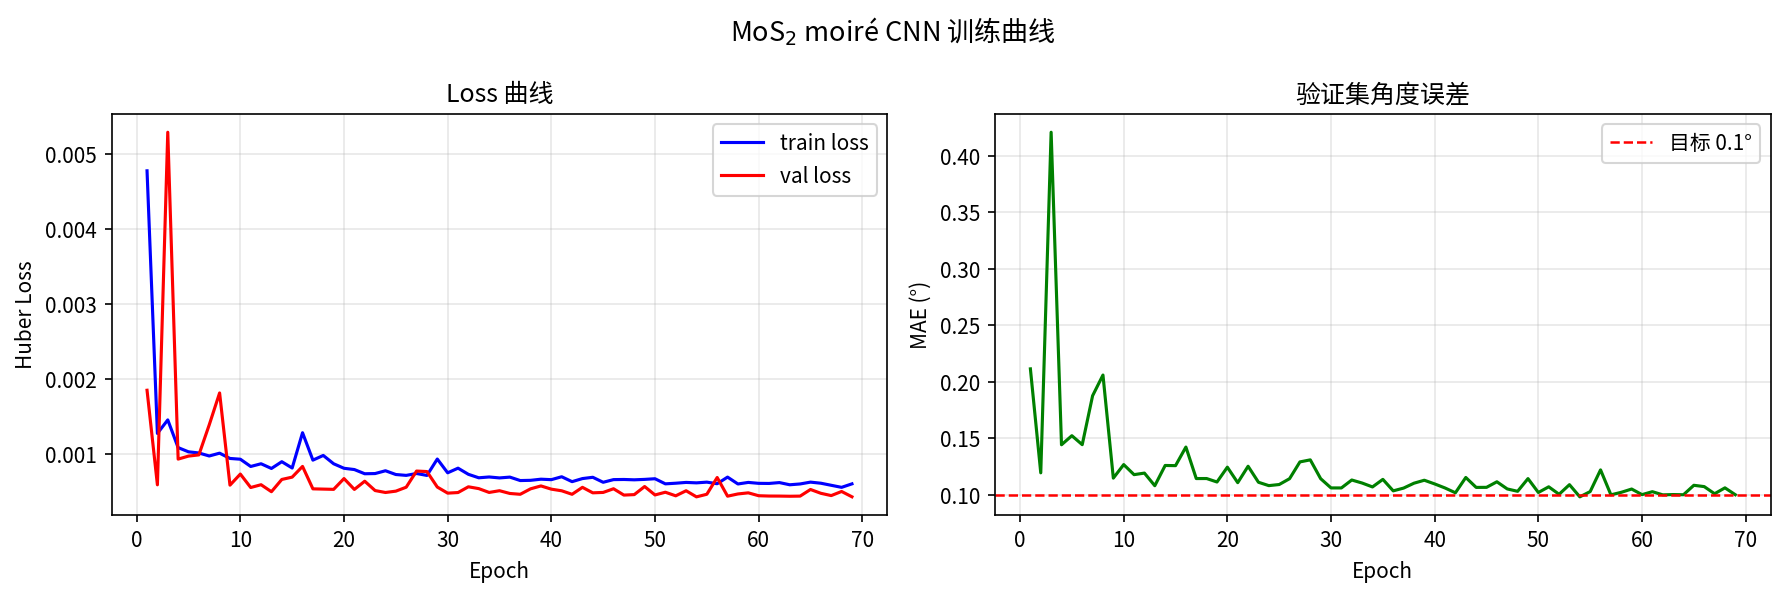
\includegraphics[width=\textwidth]{train_log.png}
\end{generalfig}

\subsection{FFT vs CNN 对比评估（公平口径）}

公平对比（\texttt{eval\_compare.py} v3）：CNN 在数据集存储的 $128{\times}128$ 三通道图上推理；FFT 则对同一标签 $\theta$ 在 $512{\times}512$ 分辨率下重新仿真高度图并施加与训练分布一致的退化，以保证 FFT 具备足够频率分辨率。这与"将 FFT 直接用于 $128{\times}128$ 测试裁剪"不同：后者视野过小会导致 moiré 峰不可靠，曾产生数度量级的伪高 FFT 误差，已在项目内分析（见 \texttt{analyze\_fft\_failure.py}）。

表~\ref{tab:final_stats} 给出当前仓库一次典型运行（测试集 $N=5000$，退化含噪声+仿射+模糊+探针卷积+$1/f$ 等）的完整统计；表~\ref{tab:comparison} 对比``公平口径''与旧``同图裁剪''口径。图~\ref{fig:compare_scatter}--\ref{fig:compare_error} 由同一评估脚本输出。

\begin{generaltab}{评测口径对照（说明历史结果与当前公平评测的差异）}{tab:comparison}
  \begin{tabularx}{\textwidth}{lXX}
    \toprule
    口径 & FFT 输入 & 说明 \\
    \midrule
    旧（易误解） & $128{\times}128$ 与 CNN 相同裁剪 & FFT 频率分辨率不足，MAE 可达数度；不宜与 CNN 直接比"谁更准" \\
    当前公平对比 v3 & $512{\times}512$ 重算高度图 & 与 graded\_eval 一致，反映"高分辨率 FFT 可走通"时的性能 \\
    \bottomrule
  \end{tabularx}
\end{generaltab}

\begin{generaltab}{FFT vs CNN 误差统计（公平对比 v3，$N=5000$，数据来自 \texttt{compare\_report.txt}）}{tab:final_stats}
  \begin{tabularx}{\textwidth}{lCC}
    \toprule
    统计指标 & FFT 方法 & CNN 方法 \\
    \midrule
    有效样本数 & 5000 & 5000 \\
    失败率 & $0.0\%$ & $0.0\%$ \\
    MAE ($^{\circ}$) & $0.0492$ & $0.0940$ \\
    中位误差 ($^{\circ}$) & $0.0281$ & $0.0761$ \\
    标准差 ($^{\circ}$) & $0.0552$ & $0.0737$ \\
    90 百分位误差 ($^{\circ}$) & $0.1264$ & $0.1992$ \\
    最大误差 ($^{\circ}$) & $0.3340$ & $0.4427$ \\
    \midrule
    MC Dropout 平均不确定度（CNN） & --- & $\pm 0.242^{\circ}$ \\
    \bottomrule
  \end{tabularx}
\end{generaltab}

在该公平设定下，FFT 的平均误差低于 CNN。这里需要强调：FFT 在当前评测口径（高分辨率重算）下误差更低，CNN 的优势主要体现在小图输入、复杂退化条件下的鲁棒性以及不确定性输出能力。真实 AFM 数据上的最终优劣仍需后续实验闭环验证。

尽管 FFT 在理想条件下精度更高，CNN 在实际应用场景中具有不可替代的优势。第一，端到端推理能力：CNN 直接从低分辨率输入（$128{\times}128$）输出角度，无需人为干预峰选择或频域后处理；而 FFT 在小视野下峰不可靠时需要人工调参。第二，退化鲁棒性：CNN 在训练过程中隐式学习了多种退化模式的联合分布，对仿射畸变、扫描行噪声等干扰天然具备更强的容忍度（distortion sweep 结果已初步验证）。第三，不确定性估计：MC Dropout 使 CNN 能在给出预测的同时量化自身置信度，为实验人员判断"该扫描是否可用"提供依据；FFT 则无内建的不确定性度量。第四，多通道融合：CNN 可同时利用 height / phase / amplitude 三个通道的互补信息，而传统 FFT 通常仅处理单一通道。第五，迁移潜力：一旦在仿真数据上完成预训练，CNN 可通过微调快速适应不同 AFM 机型或不同探针条件下的真实数据，具有更好的跨域泛化前景。

\begin{generalfig}[htbp]{FFT（左）与 CNN（右）预测值 vs 真实值（公平对比脚本输出）}{fig:compare_scatter}
  
\includegraphics[width=\textwidth]{compare_scatter.png}
\end{generalfig}

散点图（图~\ref{fig:compare_scatter}）直观展示了两种方法的系统偏差：FFT 在分辨率充足时点云更贴近理想 $y=x$，而 CNN 的离散度更大；当启用 MC Dropout 时，误差棒可视化了模型在不同角度区间的认识不确定性，为后续与 SHG 定标对齐提供了依据。

\begin{generalfig}[htbp]{误差分布与各角度区间 MAE 等（\texttt{compare\_error.png}）}{fig:compare_error}
  
\includegraphics[width=\textwidth]{compare_error.png}
\end{generalfig}

进一步地，图~\ref{fig:compare_error} 给出了误差分布直方图与按角度分箱的平均误差，可用于区分``整体 MAE''与``局部困难角度区间''。这类分解在后续真实数据迁移时尤其重要：当出现 domain gap 时，误差往往集中在特定角度或特定退化组合，而非均匀劣化。

\subsection{方法适用边界：Distortion Sweep}

脚本 \texttt{distortion\_sweep.py} 在固定其它退化量的前提下扫描仿射畸变强度，比较 FFT 与 CNN 的误差曲线（实现细节见仓库说明）。需注意：即便在部分畸变区间内 CNN 相对更稳，也不能与表~\ref{tab:final_stats} 的公平 MAE 混为一谈——二者扫描维度与汇总方式不同。结果如图~\ref{fig:distortion_sweep}。

\begin{generalfig}[htbp]{Distortion Sweep：FFT vs CNN 随畸变强度变化（由 \texttt{distortion\_sweep.py} 导出）}{fig:distortion_sweep}
  \includegraphics[width=\textwidth]{distortion_sweep.png}
\end{generalfig}

% ══════════════════════════════════════════════════════════
% 第4章  实验
% ══════════════════════════════════════════════════════════
\section{实验制备与表征}

\subsection{MoS$_2$ 机械剥离与光学表征}

采用胶带机械剥离法（Scotch tape method）从 MoS$_2$ 块材（商用高品质晶体）获取薄层片段，转移至 SiO$_2$/Si 衬底（300 nm 氧化层）。300 nm 氧化层的选择基于光学干涉增强效应，可使单层 MoS$_2$ 在白光照明下呈现明显的光学对比度，便于光学显微镜鉴别。

利用 5× 物镜（TU Plan Fluor BD，Nikon）对衬底进行系统性扫描，根据光学对比度初步筛选单层区域。单层 MoS$_2$ 的光学对比度约为 $5$--$10\%$，相比多层区域明显较低且均匀。目前正在进行单层区域的系统性搜索。

\subsection{转角同质结制备}

% 待实验完成后补充：制备过程描述、样品照片、初步转角估计结果。

计划采用撕裂-堆叠（tear-and-stack）技术制备转角 MoS$_2$ 同质结：将单层 MoS$_2$ 撕裂为两片，以 PDMS/PC 转移头拾取其中一片并旋转目标角度后堆叠在另一片上。转角由光学边缘法初步估计（精度 $1^{\circ}$--$2^{\circ}$），后续通过 AFM 和 SHG 进行精确标定。

（本节待实验完成后补充。）

\subsection{AFM 形貌表征}

计划使用华中科技大学分析测试中心 AFM 仪器进行 moiré 形貌成像；代码库中亦针对 Asylum Research Cypher ES 类输出编写了 \texttt{.ibw} 导入与平面校正、行对齐等预处理（\texttt{core/io\_afm.py}），便于与仿真 pipeline 对齐。成像参数设计如下：采用轻敲模式（Tapping mode），同时采集 Height / Phase / Amplitude 等通道；扫描范围 $200$--$500\,\mathrm{nm}$，覆盖至少 $5$--$10$ 个 moiré 周期；使用锐利针尖（前端曲率半径与仿真中 TITAN~70 设定同量级可比）以满足横向分辨率要求；数据除 \texttt{.spm} / \texttt{.gwy} 外，亦可导出为项目已支持的格式以便批处理。

实验所得到的 Height 等通道与本文仿真图像在定义与局限上的对应关系，已集中在第~\ref{subsec:afm_height_explain}~节说明：尤其应注意 Height 为 $z(x,y)$ 标量场而非``$z$ 向倒格''测量，且针尖尺度与 moiré 周期同量级时会降低条纹对比度。

（本节待 AFM 测试完成后补充实验图像及分析结果。）

\subsection{扫描探针实证参照}

为避免本文仅停留于仿真，以下引用已有扫描探针文献的实验图像作为可观测性参照（详细文献讨论见第~1.3 节）。

\begin{generalfig}[htbp]{文献实证图像示例 I：Nano Lett. 2023（STM）中不同扭角下的 moiré 纹理与频域峰，展示了与本文 FFT 管线一致的”实空间周期 + 频域峰”信息}{fig:lit_stm_moire_fft}
  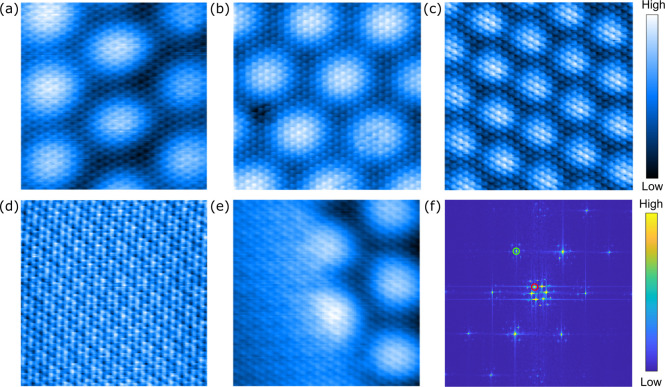
\includegraphics[width=\textwidth]{nanolett2023_fig1_stm_fft.jpg}
\end{generalfig}

\begin{generalfig}[htbp]{文献实证图像示例 II：Nat. Commun. 2020（AFM）中 MoS$_2$ 扭转样品形貌（Fig.~2），可作为本文 AFM 可行性的直接实验先例}{fig:lit_afm_liao}
  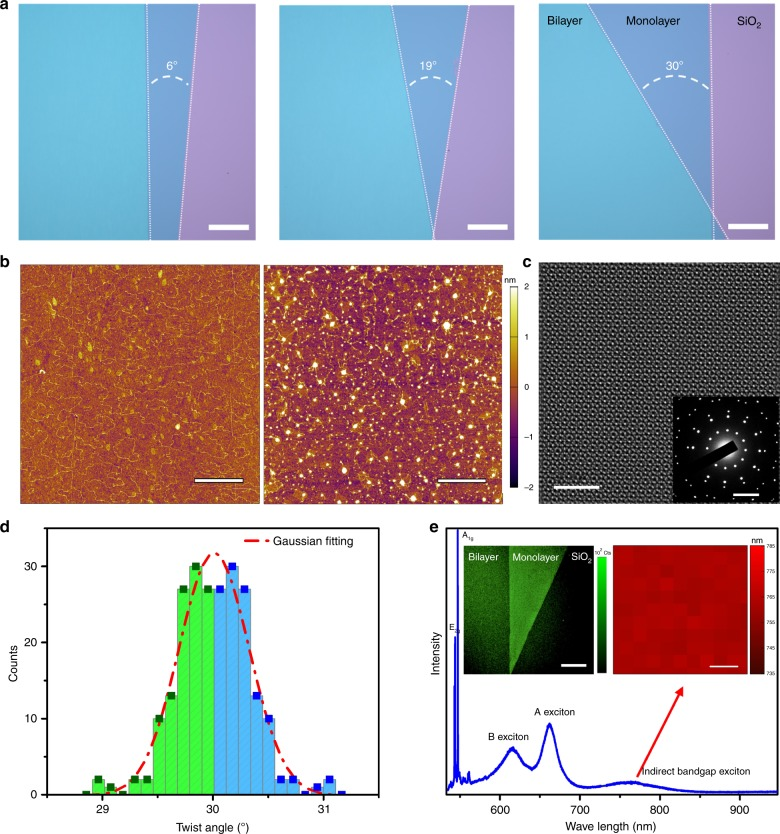
\includegraphics[width=\textwidth]{liao2020_fig2_afm.jpg}
\end{generalfig}

上述图像用于”可观测性与方法可行性”论证，而非作为本文自采样品结果。需要说明的是，上述文献与本文任务并非完全同构：本文聚焦于 Tapping 模式下 Height / Phase / Amplitude 通道的转角提取 pipeline。当前阶段属于”仿真与算法先行”，后续将以真实 AFM 数据完成迁移验证，并与 SHG 转角定标进行交叉比对。
为便于复现实证对照，项目中已整理文献图像索引与答辩说明（见 \texttt{angle\_cnn/docs/literature\_image\_benchmark.md}）。

\subsection{SHG 转角精确定标}

计划使用华中科技大学强磁场中心光学二次谐波（SHG）系统进行转角精确定标。MoS$_2$ 的 $C_{3v}$ 对称性使其 SHG 强度随入射偏振角 $\varphi$ 呈六瓣图案：
\begin{equation}
  I(2\omega) \propto \cos^2(3\varphi - \varphi_0)
\end{equation}
拟合顶层和底层各自的晶轴方向 $\varphi_0$，两者之差即为转角 $\theta$，精度优于 $0.1^{\circ}$。SHG 结果将作为 CNN pipeline 迁移验证的 ground truth。

（本节待 SHG 测试完成后补充偏振扫描曲线及定标结果。）

\subsection{CNN Pipeline 迁移验证}

获得 AFM 图像后，将对图像进行预处理（平面校正、归一化），输入训练好的 CNN 模型提取转角 $\theta_\mathrm{CNN}$，与 SHG 定标结果 $\theta_\mathrm{SHG}$ 进行比较，计算 $|\theta_\mathrm{CNN} - \theta_\mathrm{SHG}|$ 作为迁移验证误差。同时用 FFT 方法提取 $\theta_\mathrm{FFT}$，三者的对比将直接量化各方法在真实实验数据上的精度。

（本节待实验完成后补充。）

% ══════════════════════════════════════════════════════════
% 第5章  结论与展望
% ══════════════════════════════════════════════════════════
\section{结论与展望}

\subsection{主要结论}

本文围绕 MoS$_2$ 转角同质结的转角自动提取问题，建立了从物理仿真到深度学习的完整 pipeline，主要结论如下：

(1) 建立了基于 moiré 倒格矢差模型的物理仿真方法，推导了 FFT 角度提取的理论不确定度公式 $\delta\theta = a\sqrt{3}/(2\cdot\mathrm{fov})$。FFT 在频率分辨率充足、峰可辨时可达 $10^{-2}\,^{\circ}$ 量级；若仅在极小裁剪图上做 FFT，则会因视野不足产生伪高误差，需在论文与代码中与``高分辨率重算图上的 FFT''严格区分。

(2) 提出了连续晶格重构模型（strength 线性插值），消除了传统分段函数在 $\theta = 2^{\circ}$ 处的人工不连续性，与 Weston et al. 等实验观测的连续重构过渡物理图景相符\cite{weston2020atomic}。

(3) 构建了面向轻敲模式多通道、含探针卷积与多种电学/力学退化的仿真数据集，并采用改造 ResNet + Huber/Mixup 等策略训练 CNN；在公平对比（CNN 用 $128^2$、FFT 用 $512^2$ 重算）下，本次全量评测结果为 FFT MAE 约 $0.049^{\circ}$、CNN MAE 约 $0.094^{\circ}$，即该设定下 FFT 平均误差更低；CNN 仍可给出 MC Dropout 不确定性（平均约 $\pm 0.242^{\circ}$），并在畸变扫描等补充实验中与 FFT 形成互补。

(4) Distortion sweep 等实验用于刻画不同畸变强度下的相对表现，不能简单等同于表~\ref{tab:final_stats} 的全局 MAE；真实 AFM 数据上的优劣有待后续实验验证。

\subsection{展望}

后续工作主要包括以下方向：

(1) 完成实验部分：推进 MoS$_2$ 单层鉴别、转角堆叠制备、AFM 表征和 SHG 定标，以真实实验数据完成 CNN pipeline 的迁移验证。

(2) 改进仿真模型：若迁移验证误差偏大，结合真实 AFM 图像特征进一步改进退化模型，缩小 domain gap。

(3) 引入 pixel\_size 作为附加输入：当前 CNN 输入只有图像，后续可将 nm/pixel 作为额外通道输入，提升对不同扫描参数的泛化能力。

(4) 模型可解释性：通过 Grad-CAM 可视化分析 CNN 提取转角时关注的图像区域，验证模型的物理合理性。

(5) 融合估计与质量标签：为兼顾 FFT 的可解释高精度与 CNN 的鲁棒性/不确定性，后续将采用基于不确定性的动态融合
\begin{equation}
  \theta_{\mathrm{final}} = w(\sigma_{\mathrm{cnn}})\,\theta_{\mathrm{fft}}
  + \bigl(1-w(\sigma_{\mathrm{cnn}})\bigr)\,\theta_{\mathrm{cnn}},
\end{equation}
其中 $\sigma_{\mathrm{cnn}}$ 为 CNN 预测不确定度，且不确定度越大时 $w$ 越大（更偏向 FFT）。系统输出除角度估计外，还将同时给出置信区间与数据质量标签（可用/需复扫），以更好匹配实验室实际流程。

% ══════════════════════════════════════════════════════════
% 参考文献
% ══════════════════════════════════════════════════════════
\bibliography{Bibs/mybib}

% ══════════════════════════════════════════════════════════
% 附录
% ══════════════════════════════════════════════════════════
\begin{appendices}

\section{核心代码}

以下代码节选自项目仓库，为便于阅读做了格式调整，变量顺序可能与源文件不完全一致。完整代码请参见仓库中的源文件。

\subsection{连续晶格重构模型（\texttt{moire\_pipeline.py} 节选）}

\begin{verbatim}
# 连续晶格重构（无 if 硬切换）
# strength = clip(1 - theta_deg/2, 0, 1): theta=0 deg -> 1.0, theta>=2 deg -> 0.0
strength = np.clip(1.0 - theta_deg / 2.0, 0.0, 1.0)
R   = np.abs(psi)
Phi = np.angle(psi)

# R_sharp：strength=0 退化为 R（无锐化），strength=1 强锐化
R_sharp = ((1.0 - strength) * R
           + strength * np.tanh(
               strength * 8.0 * R / (R.max() + 1e-9)
             ) * R.max())

# AB/BA 两态相位量化：Im(psi) 符号区分堆叠域
domain_sign = np.sign(np.imag(psi))
phase_quant = (domain_sign + 1) / 2.0 * np.pi  # AB->0, BA->pi
Phi_recon   = (1.0 - strength) * Phi + strength * phase_quant
img = R_sharp * np.cos(Phi_recon)
\end{verbatim}

\subsection{数据集退化施加顺序（dataset\_generator.py 节选）}

\begin{verbatim}
# 退化施加顺序（对应真实成像物理过程）
# 背景倾斜 -> 方向性仿射 -> 模糊 -> 行噪声 -> 高斯噪声

# 1. 线性背景倾斜（tilt_amp: 0~30% p-p）
img = apply_background_tilt(img, tilt_amp, ax, ay)

# 2. 方向性仿射畸变（shear_x: ±0.05，shear_y: ±0.15）
img = apply_affine_distortion(img, shear_x, shear_y,
                               scale_x, scale_y)

# 3. 高斯模糊（blur: 0~2 px，针尖卷积）
img = gaussian_filter(img, sigma=blur)

# 4. 扫描行噪声（row_amp: 0~15% p-p）
row_bias = rng.standard_normal(img.shape[0]) * row_amp
img = img + row_bias[:, None]   # 水平条纹

# 5. 各向同性高斯噪声（noise: 0~50% p-p）
img = img + noise * ptp * rng.standard_normal(img.shape)
\end{verbatim}

\subsection{FFT vs CNN 公平对比报告节选（\texttt{compare\_report.txt}）}

\begin{verbatim}
MoS2 moiré：FFT vs CNN 角度提取公平对比报告
==================================================

材料：MoS2 转角同质结（a = 0.316 nm）
对比方法：
  CNN：128×128 三通道数据集图像（与训练一致）
  FFT：512×512 高度图重新生成（训练分布内退化）
退化条件：高斯噪声 + 仿射畸变 + 高斯模糊 + 探针卷积 + 1/f噪声

指标                            FFT          CNN
----------------------------------------------
有效样本数                        5000         5000
失败率                          0.0%         0.0%
MAE (°)                    0.0492       0.0940
中位误差 (°)                   0.0281       0.0761
std (°)                    0.0552       0.0737
90th pct (°)               0.1264       0.1992
最大误差 (°)                   0.3340       0.4427

MAE 比值 MAE_FFT / MAE_CNN 约 0.52（小于 1 表示 FFT 平均误差更小；以当次 eval_compare.py 输出为准）

MC Dropout 不确定性:
  平均不确定性: ±0.242°
\end{verbatim}

\end{appendices}

% ══════════════════════════════════════════════════════════
% 致谢
% ══════════════════════════════════════════════════════════
\begin{thankpage}
% 待论文完成后撰写
（致谢内容待完成后填写。）
\end{thankpage}


\end{document}
